
\chapter {HAPI}


\section{Overview}

HAPI has been designed to be a fully modular haptic rendering engine,
allowing users to easily add, substitute or modify any component of the
haptics rendering process. 

HAPI consists of the following parts:

\begin{itemize}
\item Device handling
\item Geometry based haptics
\begin{itemize} 
\item Collision handling
\item Haptics rendering algorithm
\item Surface interaction algorithm
\end{itemize}
\item Free space haptics
\begin{itemize}
\item Force effects
\end{itemize}
\item Thread handling
\end{itemize}


\subsection{Device handling}
The device handling layer provides a device independent interface for various haptics devices. It handles device initialization, cleanup, access to device state such as position and orientation and output such as force and torque. HAPI can easily be extended for new devices by implementing abstract functions for performing those tasks. See section \ref{ssAddingHapticsSupport}.

\subsection{Geometry based haptics}

\subsubsection{Haptics rendering algorithm}
A haptics rendering algorithm is need in order to calculate forces and
torques from the interaction of the haptics device with objects in the scene. An interface is provided to give a user the opportunity to implement their own
algorithm. There are four algorithms already implemented. They are:

\begin{itemize}
\item God object algorithm - point proxy based
\item Ruspini algorithm - sphere proxy based
\item Chai3D - use Chai3D rendering library
\item OpenHaptics - use OpenHaptics rendering library
\end{itemize}

Some of them have restrictions on what features of HAPI can be used, e.g. some does not support user defined surfaces. All these algorithms provide 3-DOF feedback only(i.e. no torque). 6-DOF algorithms are not currently available, however they can be generated by user force effects and rendering algoritms. Check out the details of each algorithm to find out what is supported.

\subsubsection{Collision handling}
HAPI contains classes for collision handling used in the
haptics rendering algorithms. A user have to create instances of these
classes and feed them to the haptics device that they are to be
rendered at. It also contains classes for building binary bound trees
such as axis-aligned and oriented bounding box trees from triangles,
that can be used in order to do faster collision detection. 

\subsubsection{Surface handling}
When touching the surface of a geometry, the haptics rendering
algorithm has to know what forces to generate depending on the
penetration of the surface. This is handled by the surface classes. A
user can define an arbitrary function for the force and proxy
movement (does not work for all haptics rendering algorithms though as
mentioned earlier).

\subsection{Free space haptic effects}

\subsubsection{Force effects}
Often a user wants to generate forces that are not based on
touching geometries, but instead is only depending on the state of the haptics device, such as the position and orientation. Some exampels of such effects are force fields, gravity, springs, viscosity, etc. In these cases a force effect can be used.

\subsection{Thread handling}
HAPI manages high-priority threads running at 1000 Hz for the haptics
rendering and provides mechanisms to communicate between different
threads. The thread handling functions can also be used to create new
user defined threads.      

(TODO: refer to these pictures from text either here or move to chapter about threads)

\begin{figure} 
  \centering 
  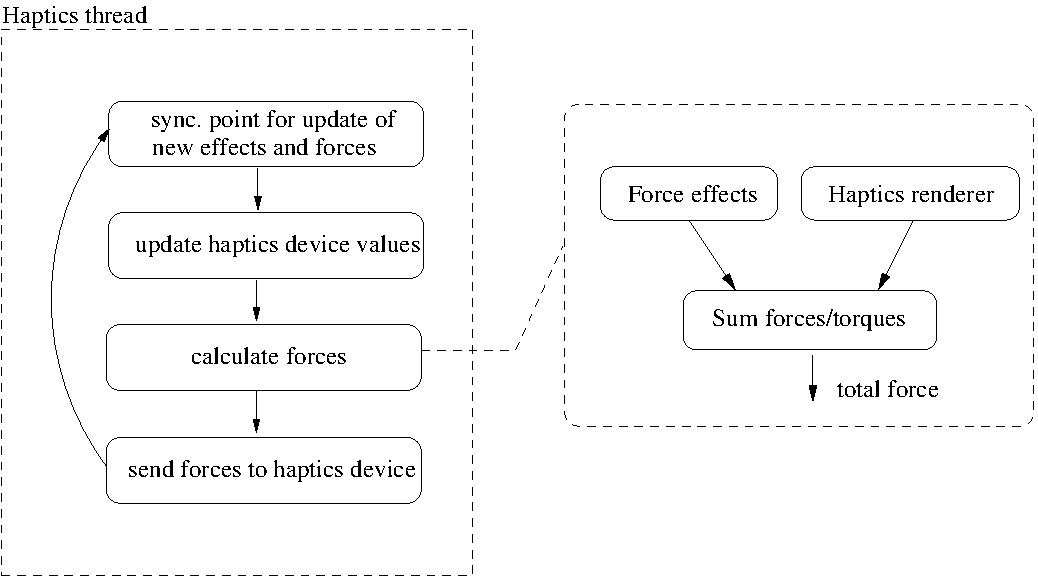
\includegraphics{images/hapticsthread.pdf}
  \caption{The flow of execution in the haptics thread.}
  \label{haptics thread} 
\end{figure}

\begin{figure} 
  \centering 
  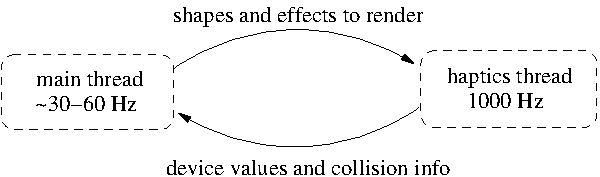
\includegraphics{images/threads.pdf}
  \caption{Thread communication}
  \label{threads} 
\end{figure}